In this section, we prove that \osgt with the set being a simple polygon is 
strongly NP-hard to approximate within a factor of $\alpha = 1.152$, through 
a sequence of auxiliary NP-hardness results. 
%
First, in Section~\ref{subsec:3regular}, we prove an intermediate result 
that the vertex cover problem is NP-complete on planar bridgeless 
$3$-regular graphs.
% 
Next, in Section~\ref{complexity:3netcomp}, starting from a planar bridgeless 
$3$-regular graph, we construct a structure which we call {\em $3$-net} and 
prove the the problem of finding the minimum coverage radius of the 
$3$-net is NP-hard to approximate within $\alpha$. 
% 
Then, in Section~\ref{subsec:osgthard}, we apply a straightforward 
reduction to transform the $3$-net into a simple polygon to complete
the hard-to-approximate proof for \osgt for simple polygons.
%

We then further show the inapproximability of the special \opgt setup 
when each robot can only guard at most two disjoint perimeter segments 
(Section~\ref{subsec:2-seghard}), contrasting the FPTAS for the special 
\opgt setup when each robot can only guard a continuous perimeter 
segment in Section~\ref{subsec:singleseg}.

\subsection{Vertex Cover on Planar Bridgeless $3$-Regular Graph}\label{subsec:3regular}
Our reduction uses the hardness result on the vertex cover problem for planar 
graphs with maximum degree $3$ \cite{garey1977rectilinear}. Such a vertex cover 
problem can be fully specified with a 2-tuple $(G, k)$ where $G = (V, E)$ is a 
planar graph with max degree $3$ and $k$ is an integer specifying the allowed 
number of vertices in a vertex cover. We note that the result has been 
suggested implicitly in \cite{mohar2001face}; we provide an explicit account 
with a simple proof. 

\begin{lemma}
Vertex cover on planar bridgeless $3$-regular graph is NP-complete.
\end{lemma}
\begin{proof}
For a given planar graph $G$ with max degree $3$ and an integer $k$,
we construct a planar bridgeless $3$-regular graph $G''$ and provide an 
integer $k''$ such that $G$ has a vertex cover of size $k$ if and only 
if $G''$ has a vertex cover of size $k''$.

\begin{figure}[ht]
    \vspace*{2mm}
    \centering
    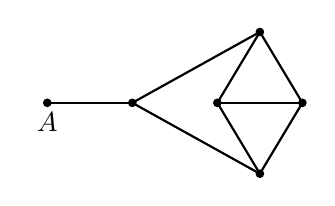
\begin{tikzpicture}[scale = .9]
        \draw[black, thick] (-0.8, 0) -- (-2,0);
        \draw[black, thick] (-0.8, 0) -- (1,1);
        \draw[black, thick] (0.4, 0) -- (1,1);
        \draw[black, thick] (1.6, 0) -- (1,1);
        \draw[black, thick] (-0.8, 0) -- (1,-1);
        \draw[black, thick] (0.4, 0) -- (1,-1);
        \draw[black, thick] (1.6, 0) -- (1,-1);
        \draw[black, thick] (0.4, 0) -- (1.6,0);
        \filldraw[black] (-0.8,0) circle (1.5pt);
        \filldraw[black] (0.4,0) circle (1.5pt);
        \filldraw[black] (1.6,0) circle (1.5pt);
        \filldraw[black] (-2,0) circle (1.5pt) node[anchor = north] {$A$};
        \filldraw[black] (1,-1) circle (1.5pt);
        \filldraw[black] (1,1) circle (1.5pt);
  			 %\node at (-2, 0) {\small{$A$}}; 
    \end{tikzpicture}
		\vspace*{2mm}
    \caption{A gadget that can be attached to a degree one or two vertices
		(at the point $A$) in a max degree $3$ graph to make all vertices have
		degree $3$. With each addition of the gadget, we increase the vertex 
		cover by a size of $3$, regardless of whether $A$ is part of a vertex 
		cover.}
    \label{fig:structure-hook}
\end{figure}

The reduction first makes $G$ $3$-regular by attaching (one or two of) the 
gadget shown in Fig.~\ref{fig:structure-hook} to $v \in G$ that are not 
degree $3$. This results in a $3$-regular graph $G'$. For each attached 
gadget, $k$ is bumped up by $3$, i.e., we let $k'$ for $G'$ be $k' = k 
+ 3(3|V(G)| - 2|E(G)|)$. It is straightforward to see that $G$ has a vertex 
cover size of $k$ if and only if $G'$ has a vertex cover size of $k'$.

\begin{figure}[!ht]
    \centering
    \raisebox{10mm}
    {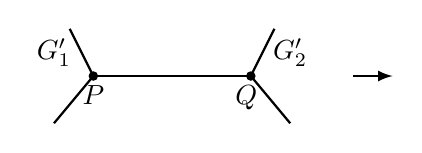
\begin{tikzpicture}
        \draw[black, thick] (-1,0) -- (1,0);
        \draw[black, thick] (-1,0) -- (-1.3,0.6);
        \draw[black, thick] (-1,0) -- (-1.5,-0.6);
        \draw[black, thick] (1,0) -- (1.3,0.6);
        \draw[black, thick] (1,0) -- (1.5,-0.6);
        \draw[black, thick, -latex] (2.3, 0) -> (2.8,0);
        \filldraw[black] (-1.5,0) node[anchor=south] {$G_1'$};
        \filldraw[black] (1.5,0) node[anchor=south] {$G_2'$};
        \filldraw[black] (-1,0) circle (1.5pt) node[anchor=north] {$P$};
        \filldraw[black] (1,0) circle (1.5pt) node[anchor=north] {$Q\,\,$};
    \end{tikzpicture}
    }
    \hfill
    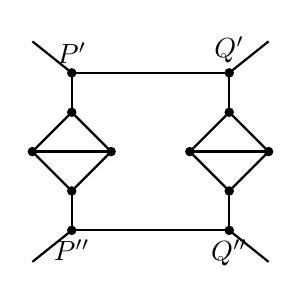
\begin{tikzpicture}
        \coordinate(p1) at (-1.5, 0);
        \coordinate(p2) at (-0.5, 0);
        \coordinate(p3) at (-1, 0.5);
        \coordinate(p4) at (-1, -0.5);
        
        \coordinate(p5) at (-1, 1);
        \coordinate(p6) at (-1, -1);
        
        \coordinate(p7) at (-1.5, 1.4);
        \coordinate(p8) at (-1.5, -1.4);

        \coordinate(q1) at (0.5, 0);
        \coordinate(q2) at (1.5, 0);
        \coordinate(q3) at (1, 0.5);
        \coordinate(q4) at (1, -0.5);

        \coordinate(q5) at (1, 1);
        \coordinate(q6) at (1, -1);
        \coordinate(q7) at (1.5, 1.4);
        \coordinate(q8) at (1.5, -1.4);
        
        \draw[black, thick] (p1) -- (p2);
        \draw[black, thick] (p1) -- (p3);
        \draw[black, thick] (p1) -- (p4);        
        \draw[black, thick] (p2) -- (p3);
        \draw[black, thick] (p2) -- (p4);
        \draw[black, thick] (p6) -- (p4);
        \draw[black, thick] (p5) -- (p3);
        

        \draw[black, thick] (q1) -- (q2);
        \draw[black, thick] (q1) -- (q3);
        \draw[black, thick] (q1) -- (q4);        
        \draw[black, thick] (q2) -- (q3);
        \draw[black, thick] (q2) -- (q4);
        
        \draw[black, thick] (q6) -- (q4);
        \draw[black, thick] (q5) -- (q3);
        
        \draw[black, thick] (q5) -- (p5);
        \draw[black, thick] (q6) -- (p6);
        
        \filldraw[black] (p1) circle (1.5pt);
        \filldraw[black] (p2) circle (1.5pt);
        \filldraw[black] (p3) circle (1.5pt);
        \filldraw[black] (p4) circle (1.5pt);
        \filldraw[black] (p5) circle (1.5pt) node[anchor=south] {$P'$};
        \filldraw[black] (p6) circle (1.5pt) node[anchor=north] {$P''$};
        
        \filldraw[black] (q1) circle (1.5pt);
        \filldraw[black] (q2) circle (1.5pt);
        \filldraw[black] (q3) circle (1.5pt);
        \filldraw[black] (q4) circle (1.5pt);
        \filldraw[black] (q5) circle (1.5pt) node[anchor=south] {$Q'$};
        \filldraw[black] (q6) circle (1.5pt) node[anchor=north] {$Q''$};
        
        \draw[black, thick] (p5) -- (p7);
        \draw[black, thick] (p6) -- (p8);
        \draw[black, thick] (q5) -- (q7);
        \draw[black, thick] (q6) -- (q8);
        
    \end{tikzpicture}
    \vspace{.5mm}
    \caption{Transformation that removes bridge $PQ$ and does not introduce new bridges.
    The minimum vertex cover number is increased by $6$ after each transformation.}
    \label{fig:rmbridge}
\end{figure}

In the second and last step, we remove bridges in $G'$. As in 
Fig.~\ref{fig:rmbridge}, for a bridge $PQ$ that divides $G'$ into $G_1'$ 
(containing $P$) and $G_2'$ (containing $Q$), we split the bridge edge 
$PQ$ using the illustrated transformation, which yields a new graph $G''$
that is planar, bridgeless, and $3$-regular, after all bridges are removed
this way. For each such augmentation, the size of the vertex cover is 
bumped up by six. Let $br(G')$ be the number of bridges in $G'$, $G'$ has 
a vertex cover of size  $k'$ if and only if $G''$ has a vertex cover 
of size $k'' = k'+6br(G')$. This completes the proof. 
\end{proof}


\subsection{Hardness on Optimally Guarding a $3$-Net}\label{complexity:3netcomp}
Starting from a planar cubic graph $G$, we construct a structure that we call 
$3$-net, $T_G$, as follows. 
%
First, similar to \cite{feder1988optimal}, to embed $G$ into the plane, 
an edge $uw \in E(G)$ is converted to an odd length path $uv_1, v_1v_2, 
\ldots, v_{2m}w$ where $m > 3$ is an integer. We note that $m$ is different
in general for different edges of $G$. 
%  to be decided later. 
Denote such a path as $u\cdots w$; each edge along $u\cdots w$ is straight 
and has unit edge length. We also require that each path is nearly straight 
locally. 
% This point will be made more precise later.
%
For a vertex of $G$ with degree $3$, e.g., a vertex $u \in V(G)$ 
neighboring $w, x, y \in V(G)$, we choose proper configurations and lengths for 
paths, $u\cdots w$, $u\cdots x$, and $u\cdots y$ such that
these paths meet at $u$ forming pairwise angles of $2\pi/3$. We denote the 
resulting graph as $G'$, which becomes the {\em backbone} of the 
$3$-net $T_G$. 

From here, a second modification is made which completes the 
construction of $T_G$. In each previously constructed 
path $u\cdots w = uv_1\ldots v_{2m}w$, for each $v_iv_{i+1}$, $1 \le i
\le 2m-1$, we add a line segment of length $\sqrt{3}$ that is 
perpendicular to $v_iv_{i+1}$ such that $v_iv_{i+1}$ and the line 
segment divide each other in the middle. A graphical illustration is
given in Fig.~\ref{fig:path-bar}. 
% We note that the bars do not need to be connected to the backbone $G'$. 
$G'$ and the bars form the 
$3$-net, which we denote as $T_G$. An example of transforming $K_4$
into a {\em 3-net} is given in Fig.~\ref{fig:3-net}.

\begin{figure}[ht]
% \vspace*{-4mm}
    \centering
		\vspace*{1mm}
    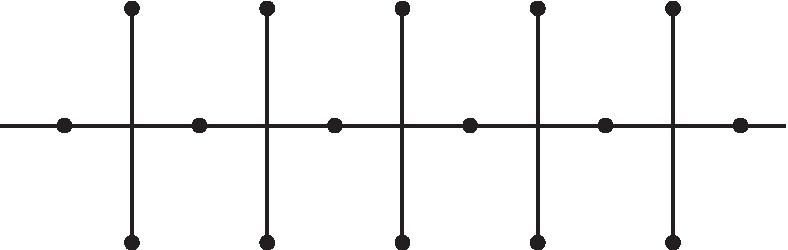
\includegraphics[scale=0.3]{chapters/osg/figures/edgepath-eps-converted-to.pdf}
		\vspace*{3mm}
% \vspace*{-4mm}
    \caption{Structure within the odd length path and attached 
		perpendicular ``bars'' with length $\sqrt{3}$. Regarding the 
		representation of such non-integral coordinates in the problem 
    input, 
    we may scale the coordinates to some certain extent and
    round them to integers so that the relative distance between
    each other is precise enough
    for the proof.
    % a precise enough fractional representation is enough 
    % for the proof due to the inapproximability gap in the result.
    }
		\vspace*{-1mm}
    \label{fig:path-bar}
\end{figure}

\begin{figure}[ht]
    \centering
    % \vspace*{-8mm}\
    \raisebox{14mm}{
    \begin{overpic}[scale=0.2]{chapters/osg/figures/k4-eps-converted-to.pdf}
      % \put(53,36){\color{black}$w$}
      \put(115,23){$\to$}
      \end{overpic}
    }
      \begin{overpic}[scale=0.4]{chapters/osg/figures/k4_after-eps-converted-to.pdf}
        \end{overpic}
    \caption{Illustration of a $3$-net obtained from $K_4$, the complete graph on 
		$4$ vertices.}
    % \caption{A $3$-net constructed over the backbone in Fig.~\ref{fig:backbone}.
        % \textcolor{red}{Siwei: update this to be based on $G'$ from Fig.~\ref{fig:backbone}}
        % }
    \label{fig:3-net}
\end{figure}

Let $L$ be the number of (unit length) edges of $G'$ (i.e., $L = 
\sum_{uv \in E(G)}len(u\cdots w)$). 
\begin{lemma}\label{l:bl}
A planar bridgeless $3$-regular graph $G$ has a vertex cover of size 
$k$ if and only if its transformed 3-net $T_G$ can be covered
by $K = k + (L-|E(G)|)/2$ circles of radius approximately $\alpha = 1.152$.
\end{lemma}
\begin{proof}
If $G$ has a vertex cover of size $k$, then we put $k$ circles of radius $1$
at the centers of the corresponding vertices in $T_G$. 
%
For each odd length path $u\cdots w$, since either $u$ or $w$ is already 
selected as the circle center, applying one coverage pattern shown
in Fig.~\ref{fig:pathcover} with $(len(u\cdots w) - 1)/2$ circles will cover 
the rest of $u\cdots w$ and all bars on it. So, the total number of circles
used is $K$ to cover all of $T_G$. 

\begin{figure}[!ht]
  \vspace*{0mm}
      \centering
      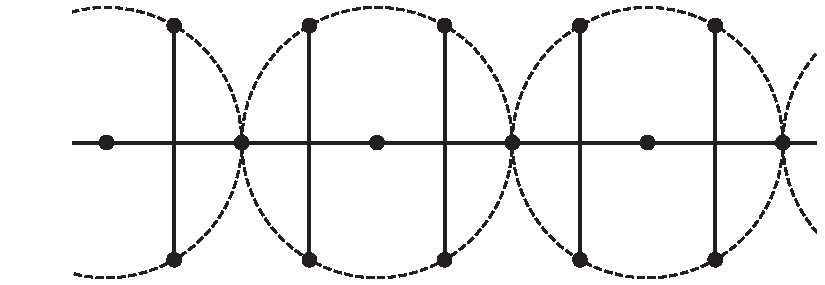
\includegraphics[scale=0.3]{chapters/osg/figures/edgepath1-eps-converted-to.pdf}\vspace{3mm}
      \hfill
      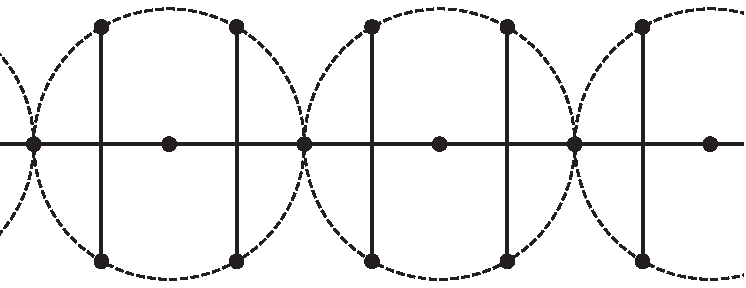
\includegraphics[scale=0.3]{chapters/osg/figures/edgepath2-eps-converted-to.pdf}
  \vspace*{0mm}
     \caption{Two coverage patterns on an odd length path with robots of 
      range sensing radius $1$ which is less than $\alpha$.}
      \label{fig:pathcover}
  \end{figure}
  
  \begin{figure}[!ht]
    \centering
    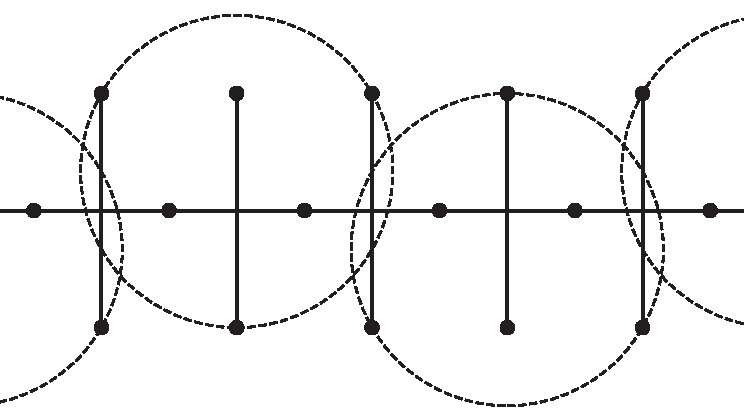
\includegraphics[scale=0.33]{chapters/osg/figures/edgepath3-eps-converted-to.pdf}
  \vspace*{1mm}
    \caption{Asymmetrical coverage of $4$ endpoints requiring a circle of 
    radius at least $2\sqrt{3}/3\approx 1.155$.}
    \label{fig:pathcovert}
  \end{figure}

The ``if'' part requires more analysis. Consider $T_G$ that can be covered 
by $K$ circles of radius $r \approx \alpha$. For a path $u\cdots w$ on $T_G$ whose 
length is $2m+1$, there are $2m-1$ vertical bars associated with it. Consider 
the $4m-2$ endpoints of these vertical bars. We note that (as shown in 
Fig.~\ref{fig:pathcovert}), it requires a radius of $2\sqrt{3}/3\approx 1.155$ 
for a circle to cover $4$ bar endpoints in an asymmetrical manner (three endpoints
on one side of the path, one on the other). Since 
we set the radius of coverage circle to be about $\alpha = 1.152$ (actually, 
between $1.152$ and $1.153$),
a circle may only cover up to $4$ bar endpoints. When a circle does cover $4$ 
bar endpoints, it must use a symmetrical coverage pattern, i.e. $4$ endpoints
on two bars, resulting in fully covering two bars. For the 
rest of the proof, we use ``circle'' to mean circles with a radius of $\alpha$,
unless otherwise stated explicitly. 

Since there are $4m - 2$ bar endpoints, it requires $m$ circles to cover all 
bar endpoints when $m \ge 3$. Moreover, at least one circle must cover $4$ 
bar endpoints by the pigeonhole principle. Fixate on such a circle $S$, which 
must have symmetric coverage, we examine the bars on one side of it, say the 
left side, assuming the path $u\cdots w$ is horizontal. If there are more 
than two bars to the left, then it is always beneficial to cover the two bars 
immediately to the left of $S$ using another circle. To see that this is the 
case, look at the two bars ($DE$ and $FH$) and the two associated unit 
length edges ($AB$ and $BC$) to the left of $S$ in Fig.~\ref{fig:two-bar}.
It can be computed that the circle $S$ to the right can cover a maximum 
length of $0.412$ of $AB$ to $A'$. Circles to the left of $S$ then must cover 
$A'B$. Let the circle covering $A'$ be $S'$. We may assume that 
$S'$ covers at least one of $D$ and $E$ (otherwise, at least one more circle 
$S''$ must be added that fall between $S'$ and $S$, in which case $S''$ 
must also cover $A'$). 

  \begin{figure}[ht]
  \vspace*{0mm}
    \centering
     \begin{overpic}[width=0.7\columnwidth]{chapters/osg/figures/two-bar-notext-eps-converted-to.pdf}
     \put(95, 31){$S$}
     \put(62.5,13){$A$}
     \put(50,22.5){$A'$}
     \put(44.3,13){$B$}
     \put(27,13){$C$}
     \put(57.5,36){$D$}
     \put(57.5,0){$E$}
     \put(41,32){$F$}
     \put(41,1.5){$H$}
     \put(14,26){$S'$}
     \end{overpic}
  \vspace*{3mm}
    \caption{When there are enough bars left, it is always better to cover
		two bars at a time with a circle. Two extremal cases of $S'$ covering
		$A'$ and $D$ but not $E$ are shown (as dashed circles), which amounts 
		to rotating the circle $S'$ around $D$.}
    \label{fig:two-bar}
  \end{figure}

If $S'$ covers $A'$ and only one of $D$ or $E$, say $D$, some other circle 
$S''$ must cover $E$. In this case, the coverage region of $S'$ and $S''$ are 
bounded by circles of radius approximately $2.304$ with center at $D$ and $E$, 
respectively. It is readily observed that $S'$ and $S''$ can reach at most one 
more bar to
the left of $FH$ (we note that $S'$ and $S''$ will not be able reach structures
on the $3$-net beyond $u\cdots w$ path). In this case, we can instead move $S'$ 
cover $A'C$, $DE$, and $FH$, and move $S''$ cover the bar to the left of $FH$ 
and potentially one more bar. Therefore, we may assume that $S'$ covers bar 
endpoints $D, E, F$, and $H$, symmetrically along the $u\cdots w$ path. 
Following the reasoning, we may assume that all bars on paths are covered, 
two at a time by a circle in a symmetrical manner, until there are one or two 
bars left before a path reaches a junction where it meets other paths. 

Because there are odd number of bars on a path, the symmetric coverage pattern 
extends until one side of a path has two bars remaining while the other side
has one bar. $m - 2$ circles have been used so far, which means that at least 
two more circles are needed to cover the remaining three bars. Without loss of 
generality, assume two bars out of these three are adjacent and are on the left 
end of $u\cdots w$ and one is on the right. Denote these bars as $b_1, b_2$, 
and $b_3$, from left to right. We call the end of a path with two bars the 
{\em even end} (e.g., the side ending with two bars $b_1$ and $b_2$) and the 
end of the path with one bar the {\em odd end} (e.g., the side ending with one 
bar $b_3$). 

We now examine the coverage of $b_2$ (see Fig.~\ref{fig:end-two-bar} where 
$b_1$ corresponds to $CD$ and $b_2$ corresponds to $AB$). Again, if the two 
endpoints $A$ and $B$ of $b_2$ are covered by more than one circle, then one 
of these two circles can be replaced with one that fully covers $b_1$ and 
$b_2$ (the solid circle in Fig.~\ref{fig:end-two-bar}), since a circle 
covering only one endpoint of $b_2$ (e.g., $B$) will not be able to reach 
structures outside $u\cdots w$. By now, $m-1$ circles have been used and to 
cover $u \cdots w$, at least two more circles are needed at the two ends 
(i.e., $m+ 1$ circles are required to cover $u\cdots w$). 

  \begin{figure}[ht]
    \centering
     \begin{overpic}[width=0.6\columnwidth]{chapters/osg/figures/end-two-bar-notext-eps-converted-to.pdf}
     \put(18, 28.5){$u$}
     \put(64.5, 43){$A$}
     \put(60, 10){$B$}
     \put(51, 39){$C$}
     \put(51, 15.5){$D$}
     \put(68,10){\rotatebox{-12}{{\small $r=2.304$}}}
		 \end{overpic}
  \vspace*{1mm}
    \caption{When there are two bars at the end of a path, it is preferred
		to cover them with a single circle (in red). The dotted circle shows that 
		a circle of radius $2*\alpha$ covering $B$ will not be able to reach 
		structures outside $u\cdots w$.}
    \label{fig:end-two-bar}
  \end{figure}


Next, instead of examining $b_3$, we examine the possible configurations at 
junctions where paths meet. There are four possible cases that contains 
$0$-$3$ odd ends. For the case where only even ends meet, one additional 
circle is needed to cover the rest of the junction 
(Fig.~\ref{fig:junction}(a)). When there is one odd end and two even ends 
(Fig.~\ref{fig:junction}(b)), it requires one more circle to cover the 
junction. This constraint is how the radius $\alpha = 1.152$ is obtained 
(more precisely, with circles with radius 1.153, no additional circles are 
needed at the junction). When there are two odd ends and one even end 
(Fig.~\ref{fig:junction}(c)), at least one more circle is needed to cover 
the the junction. For the last case (Fig.~\ref{fig:junction}(d)), no 
additional circles are needed. The cases where additional cycles are needed 
correspond to the junction vertex being selected as a vertex cover. 
It is straightforward to observe that the constructed vertex cover is a valid 
one. The cover has size of $K-(L-|E(G)|)/2$. 

\begin{figure}[!ht]
	\vspace*{4mm}
  \centering
  \hspace{-10mm}
\begin{overpic}[scale=0.66]{chapters/osg/figures/junction-eps-converted-to.pdf}
  \put(16, 0){(a)}
  \put(40, 0){(b)}
  \put(64, 0){(c)}
  \put(88, 0){(d)}
\end{overpic}
\vspace*{2mm}
  \caption{The four possible patterns at the junction using circles of radius 
	less than $\alpha = 1.152$. When we increase the radius to $r = 1.152259$, 
	circles shown in (b) and (c) can successfully cover the junction and the odd 
	ends.}
  \label{fig:junction}
\end{figure}
\end{proof}

It is clear that Lemma~\ref{l:bl} holds for discs with radius in 
$[1, \alpha)$. Thus, approximating $size(T_G, K)$ to less than a 
factor of $\alpha$ will decide whether $G$ has a vertex cover of 
$k$, yielding the hard-to-approximate result.
Also, it can be observed that all lengths are polynomial with respect to 
the problem input size, which implies strongly NP-hardness.
\begin{theorem}\label{t:3nethard}
The minimum radius for cover a $3$-net using 
% $(({L-|E|})/{2}+k)$ 
$k$ circular discs 
% while minimizing the maximum disc radius 
is strongly NP-hard to approximate within a 
factor of $\alpha = 1.152$.
\end{theorem}


\subsection{From $3$-Nets to Simple Polygons}\label{subsec:osgthard}
We proceed to show that \osgt is hard to approximate for a simply polygon 
by converting a $3$-net into one. Along the backbone $G'$ of a $3$-net 
$T_G$, we first expand the line segments by $\delta$ to get a 2D region  
(see Fig.~\ref{fig:door}(a)). We may describe the interior of the resulting 
polygon as 
\vspace*{-1mm}
\[P=\{p\in \R^2\ |\ \min_{q\in T_G}(\lVert p-q\rVert_1)\leq \delta/2\}\]
\vspace*{-4mm}

For small enough $\delta$, it's clear that $P$ is a polygon with holes.
Let $K = (({L-|E|}){2}+k)$, it holds that
\vspace*{-1mm}
\begin{align*}
&size(K, T_G) \leq               size(K, P)\leq size(K, T_G) + \delta,\\
&size(K, T_G) \leq      size(K, \partial P)\leq size(K, T_G) + \delta.
\end{align*}
\vspace*{-5mm}

To convert the structure into a simple polygon, we can open ``doors'' of 
width $\delta$ on the structure to get rid of the holes (see 
Fig.~\ref{fig:door}(b)). Each opening removes one hole from $P$. This is 
straightforward to check; we omit the details. 
\begin{figure}[ht]
		\centering
		\vspace*{0mm}
    \begin{small}
    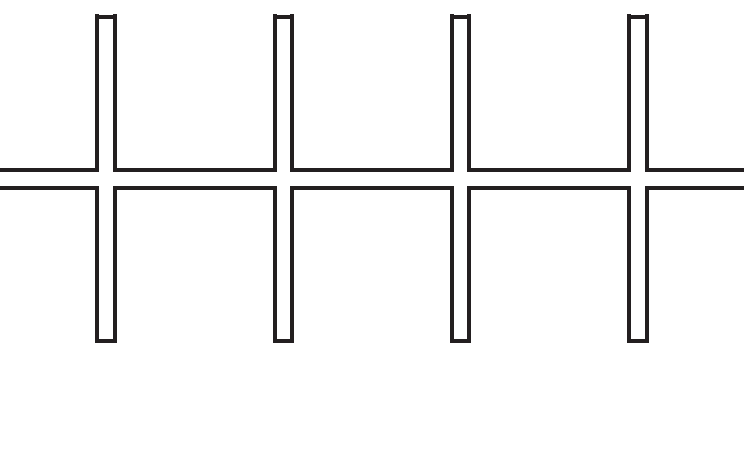
\includegraphics[scale=.3]{chapters/osg/figures/holes-eps-converted-to.pdf} 
    \hfill
    \begin{overpic}[scale=.3]{chapters/osg/figures/doors-eps-converted-to.pdf}
        \put(50,42){$\delta$}
        \put(-75,3){(a)}
        \put(46,3){(b)}
    \end{overpic}
	  \end{small}
		\vspace*{1mm}
    \caption{(a) A $3$-net $T_G$ maybe readily converted into a simple polygon 
		$P$ with holes by expanding along its backbone. (b) Creating a ``door'' 
		of width $\delta$ will remove one hole from $P$.}
    \label{fig:door}
\end{figure}

Denoting the resulting simple polygon as $P'$, we have
\vspace*{-1mm}
\begin{align*}
&size(K, P) - \delta  \leq               size(K, P')\leq size(K, P),\\
&size(K, \partial P) - \delta  \leq      size(K, \partial P')\leq size(K, \partial P).
\end{align*}
\vspace*{-5mm}

Therefore, both $size(k, P')$ and $size(k, \partial P')$ are between 
$size(k, T_G) - \delta$ and $size(k, T_G) + \delta$. Suppose the \osgt for 
$\partial P'$ or $P'$ has a polynomial approximation algorithm with 
approximation ratio $1.152 - \varepsilon$ where $\varepsilon > 0$, let $\delta = 
\varepsilon/2$, then the optimal guarding problem for the $T_G$ can 
be approximated within 1.152 disobeying the inapproximability gap by 
Theorem~\ref{t:3nethard}. Therefore,

\begin{theorem}\label{t:osgthard}
\osgt is NP-hard and does not admit a polynomial time approximation 
within a factor of $\alpha$ with $\alpha = 1.152$, unless 
P$=$NP.
\end{theorem}

\subsection{\opgt with Sensor Guarding Restrictions}\label{subsec:2-seghard}
The inapproximability gap from Theorem~\ref{t:osgthard} prompts us to 
further consider restrictions on the setup with the hope that meaningful 
yet more tractable problems may arise. On natural restriction is to 
limit the number of continuous segments a mobile sensor may cover. As 
will be shown in Section~\ref{subsec:singleseg}, if a mobile sensor may 
only guard a single continuous perimeter segment, a 
$(1 + \varepsilon)$-optimal solution can be computed efficiently. 
On the other hand, it turns out that if a sensor can guard up to two 
continuous perimeter segments, \opgt remains hard to approximate. 

\begin{theorem}\label{them:twoconthard}
\opgt of a simple polygon cannot be approximated within $\alpha\approx 1.152$ 
even when each robot can guard no more than two continuous boundary segments,
unless P$=$NP.
\end{theorem}
\begin{proof}
Due to \cite{petersen1891}, every bridgeless $3$-regular graph $G$ has a 
perfect matching. We can obtain such a perfect matching of the $3$-regular 
graph using Edmonds' Blossom algorithm in polynomial time\cite{edmonds_1965}. 
Doubling the edges in the perfect matching, we can then obtain a 4-regular 
graph $G'$. 

\begin{figure}[ht]
		\vspace*{-2mm}
    \centering
    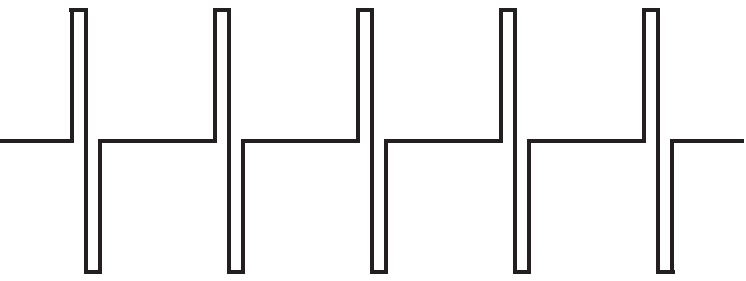
\includegraphics[scale=0.3]{chapters/osg/figures/1going-eps-converted-to.pdf}\hspace{2mm}
	  \begin{overpic}[scale=.3]{chapters/osg/figures/2going-eps-converted-to.pdf}
        \put(-55,-10){(a)}
        \put(49,-10){(b)}
    \end{overpic}
		\vspace*{6mm}
    \caption{(a) Part of the augmented Eulerian path for non-doubled 
		paths. (b) Part of the augmented Eulerian path for doubled paths.}
    \label{fig:path_exp}
		\vspace*{-1mm}
\end{figure}

The Eulerian tour on $T_G$ may have self-intersections, which 
will prevent the tour from being a simple polygon. To address this, we may use 
one of two possible solutions outlined in Fig.~\ref{fig:eliminter} to eliminate
the self-intersections. 
\begin{figure}[ht]
    		\vspace*{2mm}
				\centering
	  \begin{overpic}[width=\columnwidth]{chapters/osg/figures/t345-eps-converted-to.pdf}
        \put(12,-6){(a)}
        \put(48,-6){(b)}
        \put(84,-6){(c)}
    \end{overpic}
		\vspace*{3mm}
        \caption{In order to eliminate possible self-intersections in 
				(a), we may transform it into one of the solutions given in 
				(b) and (c) to make the Eulerian tour remain connected (one 
				of the two solutions will satisfy this).}
        \label{fig:eliminter}
\end{figure}

At this point, we readily observe that Theorem~\ref{t:osgthard} applies. 
Furthermore, an optimal solution always allows each mobile sensor to 
cover only two continuous perimeter segments. This is clear in the middle 
of any paths of $T_G$; at junctions, the polygon boundary will be either 
one of two possibilities shown in Fig.~\ref{fig:2types}, where a sensor
again covers at most two continuous segments of the simple polygon. 
\begin{figure}[!ht]
    \centering
    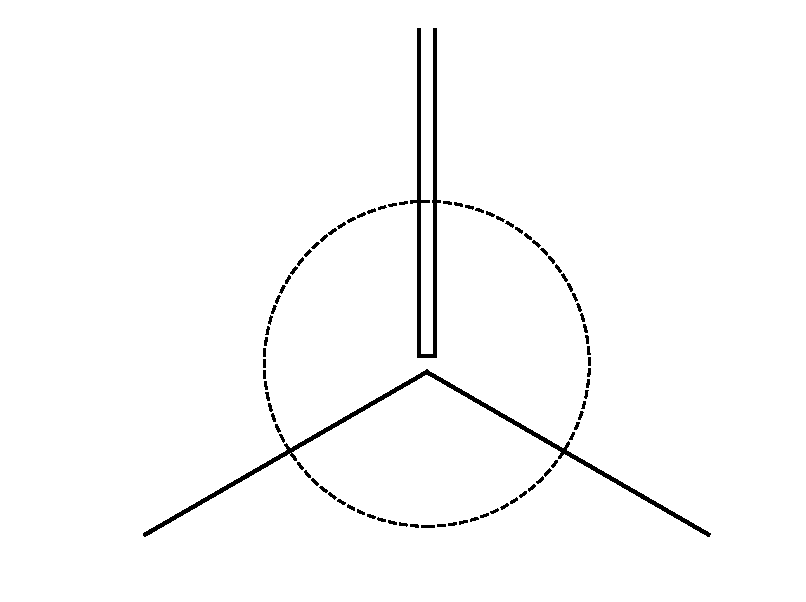
\includegraphics[scale=.29]{chapters/osg/figures/t1-eps-converted-to.pdf}
    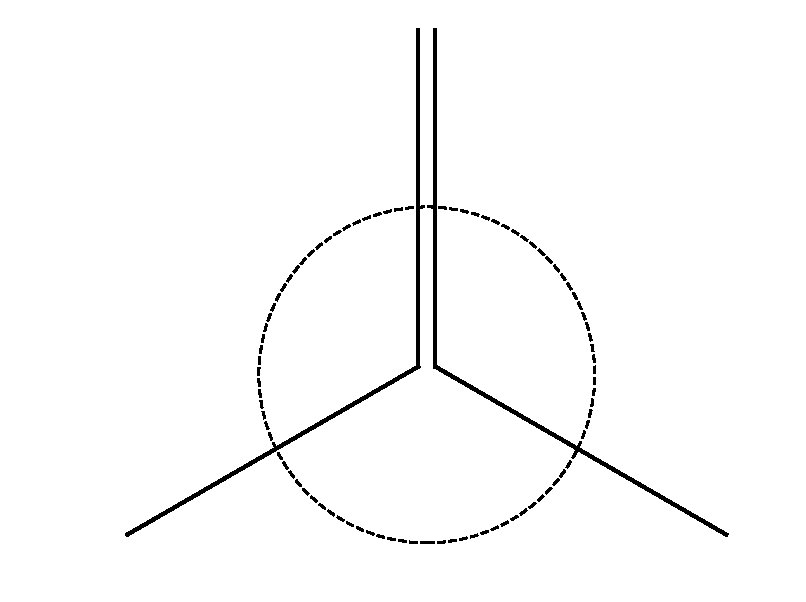
\includegraphics[scale=.29]{chapters/osg/figures/t2-eps-converted-to.pdf}
    \caption{The figure shows two possible types of boundaries near a 
		vertex with degree of $4$. A robot near the vertex will only be able 
		to cover two disjoint but individually continuous boundary segments 
		with sensing radius less than $\alpha$ if the solution is to be optimal.}
    \label{fig:2types}
\end{figure}
\end{proof}
